%  ========================================================================
%  Copyright (c) 1985-2014 The University of Washington
%
%  Licensed under the Apache License, Version 2.0 (the "License");
%  you may not use this file except in compliance with the License.
%  You may obtain a copy of the License at
%
%      http://www.apache.org/licenses/LICENSE-2.0
%
%  Unless required by applicable law or agreed to in writing, software
%  distributed under the License is distributed on an "AS IS" BASIS,
%  WITHOUT WARRANTIES OR CONDITIONS OF ANY KIND, either express or implied.
%  See the License for the specific language governing permissions and
%  limitations under the License.
%  ========================================================================
%

% Documentation for University of Washington thesis LaTeX document class
% by Jim Fox
% fox@washington.edu
%
%    Revised for version 2015/03/03 of uwthesis.cls
%
%    This document is contained in a single file ONLY because
%    I wanted to be able to distribute it easily.  A real thesis ought
%    to be contained on many files (e.g., one for each chapter, at least).
%
%    To help you identify the files and sections in this large file
%    I use the string '==========' to identify new files.
%
%    To help you ignore the unusual things I do with this sample document
%    I try to use the notation
%       
%    % --- sample stuff only -----
%    special stuff for my document, but you don't need it in your thesis
%    % --- end-of-sample-stuff ---


%    Printed in twoside style now that that's allowed
%
 
\documentclass [11pt, proquest] {uwthesis}[2015/03/03]
 
%
% The following line would print the thesis in a postscript font 

\usepackage{amsfonts,amsmath,amsthm}
\usepackage[usenames]{color}
\usepackage{mathptmx} % assumes new font selection scheme installed
\usepackage{times} % assumes new font selection scheme installed
\usepackage{amssymb}  % assumes amsmath package installed
\usepackage{tabularx}
\usepackage{graphicx}
\usepackage{dcolumn}
\usepackage{epstopdf}
\usepackage{gensymb}
\usepackage{tikz}
\DeclareGraphicsRule{.eps}{pdf}{.pdf}{`epstopdf #1}
\pdfcompresslevel=9

% Table and figure captions
% http://tex.stackexchange.com/questions/75654/uppercase-until-end-of-group


%\setlength{\oddsidemargin}{0cm} \setlength{\evensidemargin}{0cm}
%\setlength{\topmargin}{-.25cm}  % -2 works for ps but not dvi or pdf!
%\setlength{\textheight}{21.5cm} \setlength{\textwidth}{15.7cm}


% \usepackage{natbib}
% \def\bibpreamble{\protect\addcontentsline{toc}{chapter}{Bibliography}}
\def\checkmark{\tikz\fill[scale=0.4](0,.35) -- (.25,0) -- (1,.7) -- (.25,.15) -- cycle;} 

\setcounter{tocdepth}{1}  % Print the chapter and sections to the toc
 

% ==========   Local defs and mods
%

% --- sample stuff only -----
% These format the sample code in this document

\usepackage{alltt}  % 
\newenvironment{demo}
  {\begin{alltt}\leftskip3em
     \def\\{\ttfamily\char`\\}%
     \def\{{\ttfamily\char`\{}%
     \def\}{\ttfamily\char`\}}}
  {\end{alltt}}
 
% metafont font.  If logo not available, use the second form
%
% \font\mffont=logosl10 scaled\magstep1
\let\mffont=\sf
% --- end-of-sample-stuff ---
 



\begin{document}
 
%% ==========   Preliminary pages
%%
%% ( revised 2012 for electronic submission )
%%
%
%\prelimpages
% 
%%
%% ----- copyright and title pages
%%
%\Title{A Study on the Bike Volume Prediction\\
%  using EcoCounter in Seattle}
%\Author{Weiran Zhao}
%\Year{2016}
%\Program{UW Master of Urban planning}
%
%\Chair{Name of Chairperson}{Title of Chair}{Department of Chair}
%\Signature{First committee member}
%\Signature{Next committee member}
%\Signature{etc}
%
%\copyrightpage
%
%% \titlepage  
%
%% --- sample stuff only -----
%% unusual footnote not found in a real thesis
%% You just use the \titlepage as commented out above
%
%{\Degreetext{A dissertation%
%  \footnote[2]{an egocentric imitation, actually}\\
%  submitted in partial fulfillment of the\\ requirements for the degree of}
% \def\thefootnote{\fnsymbol{footnote}}
% \let\footnoterule\relax
% \titlepage
% }
%\setcounter{footnote}{0}
%
%% --- end-of-sample-stuff ---
% 
%%
%% ----- signature and quoteslip are gone
%%
%
%%
%% ----- abstract
%%
%
%
%\setcounter{page}{-1}
%\abstract{%
%This sample dissertation is an aid to students who are attempting
%to format their theses with \LaTeX, a sophisticated
%text formatter widely used by mathematicians and scientists everywhere.
% 
%\begin{itemize}
%\item It describes the use of a specialized
%macro package developed specifically for thesis production
%at the University.
%The macros customize \LaTeX\ for the correct thesis style,
%allowing the student to concentrate on the substance of
%his or her text.%
%\footnote{See Appendix A to obtain the source to this
% thesis and the class file.}
%\item It demonstrates the solutions to a variety of
%formatting challenges found in thesis production.
%\item It serves as a template for a real dissertation.
%\end{itemize}
%}
% 
%%
%% ----- contents & etc.
%%
%\tableofcontents
%\listoffigures
%%\listoftables  % I have no tables
% 
%%
%% ----- glossary 
%%
%\chapter*{Glossary}      % starred form omits the `chapter x'
%\addcontentsline{toc}{chapter}{Glossary}
%\thispagestyle{plain}
%%
%\begin{glossary}
%\item[argument] replacement text which customizes a \LaTeX\ macro for
%each particular usage.
%\item[back-up] a copy of a file to be used when catastrophe strikes
%the original.  People who make no back-ups deserve
%no sympathy.
%\item[control sequence] the normal form of a command to \LaTeX.
%\item[delimiter] something, often a character, that indicates
%the beginning and ending of an argument.
%More generally, a delimiter is a field separator.
%\item[document class] a file of macros that tailors \LaTeX\ for
%a particular document.  The macros described by this thesis
%constitute a document class.
%\item[document option] a macro or file of macros
%that further modifies \LaTeX\ for
%a particular document.  The option {\tt[chapternotes]}
%constitutes a document option.
%\item[figure] illustrated material, including graphs,
%diagrams, drawings and photographs.
%\item[font] a character set (the alphabet plus digits
%and special symbols) of a particular size and style.  A couple of fonts
%used in this thesis are twelve point roman and {\sl twelve point roman
%slanted}.
%\item[footnote] a note placed at the bottom of a page, end of a chapter,
%or end of a thesis that comments on or cites a reference
%for a designated part of the text.
%\item[formatter] (as opposed to a word-processor) arranges printed
%material according to instructions embedded in the text.
%A word-processor, on the other hand, is normally controlled
%by keyboard strokes that move text about on a display.
%\item[\LaTeX] simply the ultimate in computerized typesetting.
%\item[macro]  a complex control sequence composed of 
%other control sequences.
%\item[pica] an archaic unit of length.  One pica is twelve points and
%six picas is about an inch.
%\item[point] a unit of length.  72.27 points equals one inch.
%\item[roman]  a conventional printing typestyle using serifs.
%the decorations on the ends of letter strokes.
%This thesis is set in roman type.
%\item[rule] a straight printed line; e.g., \hrulefill.
%\item[serif] the decoration at the ends of letter strokes.
%\item[table] information placed in a columnar arrangement.
%\item[thesis] either a master's thesis or a newal dissertation.
%This document also refers to itself as a thesis, although it
%really is not one.
% 
%\end{glossary}
% 
%%
%% ----- acknowledgments
%%
%\acknowledgments{% \vskip2pc
%  % {\narrower\noindent
%  The author wishes to express sincere appreciation to
%  University of Washington, where he has had the opportunity
%  to work with the \TeX\ formatting system,
%  and to the author of \TeX, Donald Knuth, {\it il miglior fabbro}.
%  % \par}
%}

%
% ----- dedication
%
%\dedication{\begin{center}to my dear husband, Tao\end{center}}

%
% end of the preliminary pages
 
 
 
%
% ==========      Text pages
%
%
\textpages
 
% ========== Chapter 1
 
\chapter {Introduction}
 
\section{Background}
Bicycling has becoming an increasingly important transportation mode because of its: 1) non-motorized transportation nature which reduces greenhouse gas emissions, 2) ability to relieve traffic congestion and parking difficulties, 3) improved safety of all roadway users, 4) benefits to personal physical wellness, and 5) affordability and accessibility to a broader group of people. As a result, policy makers and urban planners have been consistently promoting the share of bicycling as a major substitute of automobiles in urban transportation. The city of Seattle has set forth goals to increase amount and mode share of bicycle riding in its Bicycle Master Plan (BMP). The BMP calls for a citywide network of trails, protected bicycle lanes, and neighborhood greenways, and proposes an addition of more than 35 miles of protected bicycle lanes and more than 50 miles of neighborhood greenways throughout the city in the next five years~\cite{SDOT_BMP15}.


Increasing levels of bicycle traffic create the need to quantify the use of these travel modes and their interaction with vehicles in transportation corridors~\cite{MNResearch10}. Reliable bike count estimations/predictions are essential to determine/justify whether current corridor designs are working well and for future design of appropriate infrastructure that can accommodate bicycles, pedestrians and vehicles safely. In order to better develop policy and improve relevant infrastructure planning to induce more bicycling, a robust understanding of the factors that impact bicycle volume is necessary. With the advent of automated bike counters that are now installed in multiple sites across the City of Seattle, we are now in a good position to adopt a quantitative approach to investigate the relationship of bike volume and various factors such as weather, seasons, holidays, etc. One of the objectives of this thesis is to provide an extensive study on the impact of different factors on daily bike volume. 

A robust understanding of bike volumes can be useful for policy makers, urban planners, and researchers to understand safety, travel behavior, and development needs. More specifically, it has the following impacts~\cite{LAManual} :
\begin{enumerate}
\item[-] Determine existing travel patterns and demand;
\item[-] Identify corridors where current use and potential for increased use is high;
\item[-] Track trends over time;
\item[-] Evaluate the effectiveness of programs and/or facilities to promote biking;
\item[-] Identify locations for bicycle facility improvements and design appropriate treatments;
\item[-] Measure demographic changes as facilities that increase user comfort and attract a wider range of pedestrians and bicyclists are developed;
\item[-] Assess future bicycle travel demand;
\item[-] Make informed transportation decisions to prioritize bicycle improvement projects;
\item[-] Appropriately allocate resources for active transportation.
\end{enumerate}

\section{Objectives and contribution of this thesis}
There are three major objectives that are addressed in this thesis:
\begin{enumerate}
\item \textbf{Provide an extensive study on the relationship between various factors (such as weather, season, etc) and daily bike ridership counts at Fremont Bridge in the CIty of Seattle.} A systematic approach is adopted to select the factors that have most signficant impact on daily bike counts. Also, the nonlinear relationship between weather and bike counts that has been observed in the literature~\cite{} is explicitly examined and accounted for. The resulted model is interpreted both qualitively and quantitatively. 
\item \textbf{Develop a predictive model to estimate daily bike volume based on weather forecast and other temporal factors.} One benefit of this predicative model is to help transportation administrator to make better-informed decisions/preparations in case of inclement weather or special holidays that would result in siginificant change in bike counts. It is also believed to be able to help reveal multiple aspects of planning implications, such as ability to measure return on investment in bicycle facilities and help identify locations for new facilities.
\item \textbf{Understand rider behavior at the aggregated level and determine the `real' bicycle trip trend after excluding the effect of weather and other temporal/seasonal variations.} This study is useful to help determine the current travel patterns/demand, and justify the effectiveness of current and future investments in facilities to promote biking.
\end{enumerate}

The main contribution of this thesis are as follows:
\begin{enumerate}
\item \textbf{A square root transformation is applied to address the heteroscedascity in the bike counts data, and counterfactual simulations are conducted to interprate model results}. Even though there is obvious heteroscedasticity (i.e., varying variance) in the bike count data, the log transformed linear regression model is predominatly used in the literature~\cite{}, possibly due to its convenience in  model interpretation (one percent change in the independent variable results in certain fixed amount of percent change in the dependent variable). The square root transformation, well known for its ability to stablize variance~\cite{}, however does not offer straightforward interpretation as with the log-linear model. To address this, counterfactual simulations~\cite{} are conducted to help interprate the model and visualize the effect of changing one varialbe while controling others. 
\item \textbf{Explicitly examine and quantify the nonlinear relationship between weather factors between daily bike volume}. It has been noticed that there are nonlinear relationships between weather and bike volume~\cite{}. However, such nonlinearity has not been explictly modelled and their effects are mostly analyzed using exploratory data analysis. In this thesis, we adopt an Gaussian Additive Mixture approach to model the nonlinear relationship and investigate its impact on the variable selection and model specification.
\item \textbf{Interaction terms are considered as prediction variables in the regression model}. There are limited number of papers that have included interaction terms in their modeling. In those do consider, attentions are only devoted to certain interactions between humidity and temperature~\cite{}, or temperature and wind speed~\cite{}. In this thesis, we extend interaction terms to include combination of weather and temporal variables (e.g., precipitation probability and weekend) and compare their goodness-of-fit metrics.
\item \textbf{To better capture the autocorrelation in the bike count time series, an Autoregressive Integrated Moving Average (ARIMA) model is fitted and used to predict bike volumes in the future}. With the exception of very few papers~\cite{}, the majority in the literature assume the daily bike ridership count is independent. In order to develop a good predictive bike volume model, we fit an ARIMA model to account for possible autocorrelation in the daily bike counts. The accuracy of the resulting model is validated using historical data.
%\item \textbf{Quantitatively characterize the bike ridership growth trend in the past three years}
%\item \textbf{Continuous vs. Categorical}
%save for later:  When other factors were held fixed, a 43\% to 50\% increase in ridership could be expected as the temperature doubled; however, the temperature had a negative effect when it was higher than 28$^{\circ}$C and humidity was greater than 60\%. 
%A time series-based model is developed to account for seasonality as well as other cyclical trend of different levels (yearly, weekly and daily).  
\end{enumerate}
 
\section{Organization of the Thesis}
The remainder of this thesis is organized as follows: Chapter 2 surveys existing literatures on bicycle volume modeling. Methodology of the current study appears in Chapter 3. Detailed analysis and results are presented in Chapter 4, including exploratory data analysis, variable selection, model fitting and interpretation, prediction and trend analysis. Conclusions and future directions are provided in Chapter 5.
 
% ========== Chapter 2
 
\chapter{Literature Review}

Bicycling volume in cities is useful for practitioners and researchers to understand safety, travel behavior, and development impacts. Therefore the relationship between bicycle volume and various factors, with the goal to build a predictive model based on this relationship, has been of great interest to researchers over the last decade (e.g. \cite{Griswold:2011aa,Fields:2012aa,Niemeier:1996aa,Nosal:2014aa}). In the following, we first summarize existing literature from three perspectives: data source, factor selection, and methodology. Then we will provide a review of six papers that are most relevant to this thesis: Niemeier 1996.



\section{Data source}

There are two types of data sources than are commonly used: 1) Survey/census data are more used to explain influencing factors such as physical, demographical and socio-economic factors on mode choice~\cite{Parkin:2008aa,Helbich:2014aa}; 2) Self-collected bicycle count data (automatic or manual) are used to continuously tracks and records bicycle counts at a specific location over a long period of time~\cite{Griswold:2011aa, Nosal:2014aa, Miranda-Moreno:2011aa, Thomas:2009aa}. Supplemented with weather, temporal and other factors, the collected count data is suitable for developing explanatory/predicative statistical models.  

\section{Factor Selection}

A literature review accompanying a recent report by \cite{Bassok:2011aa} identified eleven primary indicators. These included 
time of day \cite{Schwartz:1999aa}, season \cite{Niemeier:1996aa}, population and employment densities \cite{McCahil:2008aa,Pinjari:2009aa}, land-use mix \cite{Pinjari:2009aa}, bicycle facility type \cite{Hunt:2007aa},
traffic volume \cite{McDonald:2007aa}, rain and temperature \cite{Niemeier:1996aa,Parkin:2008aa}, income \cite{Turner:1998aa}, and age \cite{Hunt:2007aa}. This section outlines the key points made in the literature that are
relevant to some of most important variables. 

Research has found the variability for counts has a positive association with high temperature and low precipitation~\cite{Niemeier:1996aa,Parkin:2008aa}. Meanwhile, as suggested by \cite{Lewin:2011aa} and \cite{Thomas:2009aa}, the effects of precipitation and temperature on bicycle volumes are nonlinear. For example, bicycle traffic can decrease in both very cold and very hot weather as noted by \cite{Richardson:2000aa}. Apart from the usual temperature and rain variables, \cite{Miranda-Moreno:2011aa} finds humidity and additional precipitation variables including the presence of rain in the morning and/or during the previous three hours to be significant too. Other comparative studies are also available where bicycle counts are conducted in different cities, and different sensitives to weather are examined \cite{Rose:2011aa}. As for longitudinal studies, \cite{Niemeier:1996aa} finds increased variability for counts conducted in the later months of the year. \cite{Jones:2010aa} conclude that morning peak hours from 6 AM to 9 PM accounts for a consistent 95\% of the total bicycle volumes by hourly count data. 

\section{Existing literature on weather factor selection}
In \cite{Nosal14}, a model is developed to use deviations in daily weather conditions from average conditions to predict deviations in daily cyclist totals from the average daily total. \textbf{Add a couple of sentences to evaluate its strength and weakness}

\section{Modeling Methods}

The simple linear regression model has been used in several applications \cite{Jones:2008aa,Jones:2010aa}. Other modeling approaches include \cite{Miranda-Moreno:2011aa} which develops a count model and \cite{Thomas:2009aa} which develops a time-series model. \cite{Niemeier:1996aa} also uses a Poisson model to statistically confirm  many of the factors thought to influence cyclists. The work by \cite{Gallop:2012aa} adopts a similar time-series approach while incorporating an autoregressive integrated moving average (ARIMA) analysis. 


A summary of findings from the literature are presented in Table \ref{tb:lit}. These literature together suggest an opportunity for further model development base around long-term automated counts utilizing appropriate statistical methods. How seasonal factors influence bicycle flow needs to be examined in data that last more than a year. One limitation present in much of the past literature is that few discuss goodness of fit of their modeling. Further a model that can better describe and forecast the bicycle count in longitudinal form is necessary to be developed. Models for count data with better estimation methods offer some promise. 

\begin{center}
\begin{scriptsize}
 \begin{tabular}{p{3cm} p{7cm} p{5cm}} 
 \hline
 Source & Variable(s) identified & Methods \\ [0.5ex] 
 \hline\hline
\textbf{Fields-2012} & Average daily temperature; Total weekly precipitation & Identify patterns through scatter plots; No explicit model is established. \\
  \textbf{Gallop-2012} & Temperature, Relative humidity, wind speed, visibility, fog, precipitation & Use ARIMA to account for serial correlation patterns \\
  \textbf{Griswold-2011} & Nearby population and employment density, proximity to downtown/freeway, age, education level, income, etc. & Log linear ordinary least squares regression is used to estimate a bicycle count model \\
  \textbf{Helbich-2014} & Daily maiximum air temperature, daily average wind speed, daily precipitation & Place-specific associations of weather conditions are explored through geographically weighted logit models \\
  \textbf{Hunt-2007} & Descriptive variables indicating lane use, secured parking, level of experience, etc. & Logistic model of cycling-related choices \\
  \textbf{Jones-2010} & Length of bicycle network, employment density, population density & Standard ordinary least squares regression \\
  \textbf{Lewin-2011} & Max temp, rain flag, snow flag, weekend flag, over 90 flag & Standard linear regression model \\
  \textbf{McCahil-2008} & logarithmic choice measure, population density, worker density & A new space syntax theory is used to evaluate and predict the bicycle volume throughout a network \\
  \textbf{Miranda-Moreno-2011} & Temperature, percent humidity, rain presence, rain presence in prev. 3hrs, warm \& humid, morning rain & Both log-linear model and negative binomial model are tested \\
  \textbf{Niemeier-1996} & Morning flag, rain flag, high temp flag, location variable, season variable & A Poisson count model is assumed and fitted \\
  \textbf{Nosal-2014} & Temperature, percent humidity, rain flag, rain prev. 3hrs, am rain, pm rain & The relationship is analyzed using a log-linear regression model \\
  \textbf{Parkin-2008} & Gender, car ownership, hilliness, off-road routes proportion & A logistic regression model of relevant socio-economic and physical variables is estimated. \\
  \textbf{Pinjari-2009} & Household density, employment density, fraction of commercial land area, demographic factors including proportion of population that are seniors and proportion of population by race & The model system takes the form of a joint mixed Multinomial Logit–Multiple Discrete-Continuous Extreme Value (MNL-MDCEV) structure \\
  \textbf{Rose-2011} & Temperature, rainfall, holiday flag, school season flag, day of the week & Weather and other effects examined using an aggregate model of daily ridership \\
  \textbf{Thomas-2009} & Temperature, sunshine, precipitation, wind force, cycle path use & A bi-level structure is developed with the upper level being a log-linear model and the lower level being a linear model \\ [1ex] 
 \hline
\label{tb:lit}
\end{tabular}
\end{scriptsize}
\end{center}


% ========== Chapter 3
 
\chapter{Methodology}

%\section{Methodology}

In order to discern the relationship between bicycle counts and several identified weather, seasonal, and temporal factors, we
developed a statistical model that attempts to predict daily bicycle counts from these other factors. The major contributions of this thesis are: 1) to provide a detailed analysis on the impact of various weather factors on bike counts, and 2) to quantitatively investigate the nonlinear relationship between weather factors and bike counts. This section describes the methods
and procedures we used to collect and process the raw datasets (including both bike counts and weather variables), as well as the statistical tools used for bike count modeling (including linear regression, general linearized model, Gaussian Additive Mixture model, and ARIMA time series analysis). 

\section{Study Location}
The bike facility of interest is the Fremont Bridge in the City of Seattle. The Fremont bridge crosses the Lake Washington Ship Canal and links the Fremont with the Queen Ann neighbourhood. The reason for picking Fremont bridge as our study location is: 1) A permanent, automatic bike counter is installed at the Fremont bridge, which provides continuous bike counts; 2) As opposed to other recreational facilities, the Fremont Bridge represents one of the busiest utilitarian facility in the City of Seattle, which is the subject of this thesis; 3) The bike counter on Fremont bridge was first installed in October 2012, the earliest site among the nine bike counters in Seattle, and therefore provides a rich dataset of a little more than 3 years; 4) It's relatively close to the University of Washington, and connects the northen part of Seattle to its downtown area. 5) It captures a substantial amount of bicycle traffic due to its status as one of only five facilities that carry bicyclists across the canal separating the northern and southern halves of Seattle.

SDOT has nine bike counters (four of which also count pedestrians) located on neighborhood greenways, multi-use trails, at the Fremont  Bridge and on SW Spokane Street. The counters help create a ridership baseline that can be used to assess future years and make sure the right amount of resources are invested so that the goal of quadrupling ridership by 2030 could be achieved~\cite{SDOT_BMP15}

While only 3 percent of downtown Seattle’s 200,000 daily commuters now bicycle, the number of bike commuters has increased 18 percent since 2010, according to a survey done for the Downtown Seattle Association~\cite{}, the city’s Department of Transportation and King County Metro.

\section{Data collection, processing and description}

\subsection{Bike Count Data}
Bicycle counts were collected at Fremont bridge continuously by the City of Seattle using an in-sidewalk counter manufactured by EcoCounter (see Figure~\ref{fig:ecoCounter}). When a bicycle passes over an induction loop embedded in the sidewalk on either side of the Fremont Bridge, the counter
registers the bicycle. Data from this equipment has been used in a wide range of studies, and when operating properly, the absolute error of these counters has been shown to be below 4\%~\cite{Nordback09}. Bicyclists may legally choose to ride in the roadway instead of the sidewalk, and would thus not be detected by the counter. However, we believe these crossings are rare at this location due to the design of the facility, which directs bicyclists to enter the sidewalk, and from our own experience riding and observing other riders. The counters upload data once a day at 5 am, which is then aggregated into 15 minute intervals by the City of Seattle, and are made available to the public via the City of Seattle's data portal \cite{City-of-Seattle:aa,City-of-Seattle:ab}.

\begin{figure*}
   \includegraphics[width=1\textwidth]{figures/FremontBikeEcoCounter.jpg} 
  \caption{EcoCounter on the Fremont Bridge}
  \label{fig:ecoCounter}
\end{figure*}

The bike count data used in this study cover a period of three years spanning from October 31, 2012 to October 30, 2015. The continuous bike count data is aggregated into daily counts. Note that in the literature, there is also studies on bike count modeling using hourly bike count. However, the daily bike counts are favored in this study because: 1) it carries less autocorrelation than the hourly data; 2) it's intuitive and simple to interprate, 3) we believe for bicyclists commuting to work, they make the decision of riding based on the daily weather, as opposed to the recreational riders is more likely to make deicions on a hourly basis. 

\subsection{Weather Data}
Weather data are collected by a variety of sources and are aggregated by Forecast.io. These data are available through the company's web services API \cite{The-Dark-Sky-Company:aa}. Historical daily summaries are available for a range of weather variables including several specifically important to our model such as precipitation, daily minimum and maximum temperatures, sunrise, and sunset, etc.

We downloaded and processed these data programmatically using the R programming language along with several add-on packages \cite{Grolemund:2011aa,Wickham:2011aa,Couture-Beil:2014aa,Lang:2014aa,R-Core-Team:2014aa}. Bicycle counts were aggregated by day, and then joined to weather data by date. 

\subsection{Temporal Data}
In addition to the variables collected from the above-mentioned two sources, we were also interested in controlling for holidays and whether or not the nearby University of Washington was in session. These data were collected and coded manually from the National Holiday calendar as well as the University of Washington's historic academic calendar.

\begin{figure}
  \centering
    \includegraphics[width=0.5\textwidth]{figures/daily_hist} \hfill
    \includegraphics[width=0.5\textwidth]{figures/daily_tscount_plot}
  \caption{Descriptive visualization of bicycle counts dataset.}
  \label{fg:descriptives}
\end{figure}


\section{Exploratory Data Analysis}
Figure~\ref{fg:descriptives} provides a visual summary of the processed counts data. Some apparent outliers are visible at the rightmost portion of the histogram. The two highest counts occurred the Monday and Tuesday preceding the beginning of National Bike to Work Month. And the third highest count occurred on National Bike to Work Day.

\section{Ordinary Least Squares Regression}
The ordinary least squares (OLS) regression is one of the most widely used techniques in Statistics to estimate the unknown parameters. The goal is to minimize the differences between the observed responses and the predicted response given by the linear approximation of the data. The basic linear regression model assumes the following structure:
\begin{equation}
Y = \alpha + \beta X + \epsilon, \label{eqn:olsregression}
\end{equation}
where $Y$ is the response variable (or observations, dependent variable), and $X$ is the predictors (or regressors, independent variables), $\alpha$ and $\beta$ are the unknown parameters to estimated, and $\epsilon$ is the unobserved scalar random variables (errors) which accounts for the discrepancy between the actual observed responses $Y$ and the predicted responses $\alpha + \beta X$.  

The OLS techinque offers a mathematically convinient tool to estimate the linear regression model parameters $\alpha$ and $\beta$. There are many available software packages to provide solutions to the linear problem~\eqref{eqn:olsregression}, i.e., the \texttt{lm} function in \texttt{R}. However, to properly apply the OLS estimators, certain assumptions need to be checked beforehand, such as: 1) No linear dependence (no multicolinear), 2) Strict Exogeneity ($E[\epsilon|X]=0$), 3) Homoscedasticity ($E[\epsilon^2|X]=\sigma^2$), and 4) Normality (the error term has a normal distribution). For more details on OLS regression models, readers are referred to~\cite{}.

The goodness-of-fit of the considered model is often evaluated with the $R^2$ (R squared, or the coefficient of determination) and adjusted $R^2$. The $R^2$ measures the percentage of the response variable variation that is explained by a linear model, or equivalently
\begin{equation}
R^2 = 1- \frac{\text{Residual Sum of Squares}}{\text{Total Sum of Squares}}.\label{eqn:R2}
\end{equation}
The adjusted $R^2$ adds a correction for the number of estimated parameters to guard against overfitting. Other important goodness-of-fit criterions that are used in this study are the Akaike Information Criterion (AIC) and the Bayesian Information Criterion (BIC). Details on the latter two can be found in~\cite{}.

\section{Generalized Linear Model (GLM)}

\section{Generalized Additive Mixture (GAM) Model}
\label{sec:gamintro}
The generalized additive model (GAM) is a generalized linear model in which the linear response variable depends on unknown smooth functions of the independent variables~\cite{Wiki}. The goal is to provide characterization about these smooth functions. GAM was first proposed in~\cite{Hastie86}	 to blend the properties of generalized linear models with additive models. 

Following a similar approach with the GLMs, an exponential family distribution (could also be Poisson, normal, negative binomial, etc) is specified for response $Y$ along with a link function $g$ relating the expected value of $Y$ to the predictors $X_i$ such as
\begin{equation*}
g(E[Y]) = \beta_0 + f_1(X_1) + f_2(X_2) + \hdots + f_m(X_m)
\end{equation*}
The function $f_i(X_i)$ may be specified parametric functions (e.g., polynomial) or may be specified non-parametrically, or semi-parametrically, simply as 'smooth functions', to be estimated by non-parametric means. The nonparametric GAM provides a very general modular estimation method capable of using a wide variety of smoothing methods to estimate the $f(X)$. The advantage of non-parametric models is that they are easy and efficient to fit, while the disadvantage is the inability to control the complexity of the model (degree of smoothness of $f(X)$), which often gives rise to problems with interpretation. Overall, a well calibrated GAM is likely to perform better than nearly any other model type, if the dataset is large enough and its behavior is complex enough. However, it could also have problems of overfitting as the number of smoothing parameters increases. 

In this thesis, we use the GAM model to explore the potential relationship between the dependent variable bike counts and weather factors (i.e., temperature and precipitation). It is noticed in other studies~\cite{} that the temperature has a positive effect on ridership when its below, and a negative impact when higher than. Also, the temperature squared is often used in the literature~\cite{} to account for the nonlinearity without good explanation. The GAM provides a good starting point to investigate such nonlinear relationship since it explicitly models the dependent variable on a smooth function of the independent variable. Consequently, resulting non-parametric smooth function provides valuable insight on how to include nonlinear terms in the recommended model. In this thesis, the \texttt{gam} in \texttt{R} is used to fit generalized additive models, specified by giving a symbolic description of the additive predictor. \texttt{gam} uses the backfitting algorithm~\cite{} to combine different smoothing or fitting methods. The default built-in nonparametric smooth splines are used to fit the model. 

\section{Autoregressive Integrated Moving Average (ARIMA) Model}
\label{arimaintro}

%In this section, we review the Autoregressive Integrated Moving Average (ARIMA) methodology for bicycle count time series analysis. The ARIMA model is a generalization of the Autoregressive Moving Average (ARMA) model. The biggest difference between ARIMA and ARMA is that ARIMA use the differencing step (corresponding to the 'integrated' part of the model) to reduce the non-stationarity (where ARMA requires stationarity). As the name suggested, the ARIMA methodology is comprised of three major components: differencing, autoregressive models, and moving average model.
%
%\subsection{Stationarity and Differencing}
%
%The first step in ARIMA modeling usually involves making the time series stationary. A time series is stationary if its statistical properties are all constant over time. A stationary time series has no trends, its variation and its mean have a constant amplitude, and it wiggles in a consistent fashion, i.e., its short-term random time patterns always look the same in a statistical sense. For example, time series with trends, or with seasonality, are not stationary: the trend and seasonality will affect the value of the time series at different times. On the other hand, a white noise series is stationary. In general, a stationary time series will have no predictable patterns in the long-term. 
%
%To test the stationarity of a time series, one can first observe the time series plot to check if there is an obvious trend/seasonality in the data, if the variance and mean stay constant in the long run. The Autocorrelation Function (ACF) plot is also useful to identify non-stationary series. The ACF plot depicts the autocorrelation between the $y_t$ and its lagged values $y_{t-k}$ for different values of k. By definition of stationarity, for a stationary time series, its ACF will drop to zero relatively quickly, while the ACF of non-stationary data decreases slowly.
%
%It is common that the original time series is non-stationary, but by differencing, perhaps in conjunction with some nonlinear transformation (such as taking the logarithm to stabilize variance) the time series can be made stationary. The first-differenced time series is the change between consecutive observations in the original series, and can be written as:
%\begin{equation}
%y'_t = y_t - y_{t-1}
%\end{equation}
%Occasionally the first-differenced data will not appear stationary and it may be necessary to difference the data a second time to obtain a stationary series:
%\begin{equation} 
%y''_t = y'_t - y'_{t-1} = y_t -2 y_{t-1} + y_{t-2}
%\end{equation}
%
%There are two popular statistical tests than can be used to determine whether differencing is required: the Augmented Dickey-Fuller (ADF) test and the Kwiatkowski-Phillips-Schmidt-Shin (KPSS) test. Both tests are available in R. 
%
%\subsection{Autoregressive model}
%
%The second part of the ARIMA model is the autoregressive model (or self-regressed model). A pure autoregressive model, the dependent variable (or the predictor) $y$ consists only of lagged values of itself. In other words, we forecast y using a linear combination of past values of the variable. The mathematical expression for the autoregressive model is as follows:
%  \begin{equation}
%y_t = c + \phi_1 y_{t-1} + \phi_2 y_{t-2} + \hdots + \phi_p y_{t-p} + e_t,
%\end{equation}
%where $c$ is the constant and $e_t$ is the white noise. We refer to this as an AR($p$) model.
%
%\subsection{Moving average model}
%
%Instead of using the lagged values of the forecast variable in a regression, a moving average model uses the past forecast errors in a regression-like model. Its mathematical expression is as follows:
%  \begin{equation}
%y_t = c + e_t + \theta_1 e_{t-1} + \theta_2 e_{t-2} + \hdots + \theta_q e_{t-q},
%\end{equation}
%where $e_t$ is the white noise and the model is referred to as MA($q$). It means that each value of $y_t$ can be thought of as a weighted moving average of the past few forecast errors. Note that $e_t$ cannot be directly observed and it can only be computed on a period-to-period basis when the model is fitted to the data. Therefore, the error terms in MA($q$) are not independent variable like the normal linear regression models and solving MA($q$) requires nonlinear optimization methods rather than by just solving a system of equations.
%
%\subsection{Non-seasonal ARIMA model}
%
%By combining the above three components: differencing, autoregressive model and the moving average model, we have the non-seasonal ARIMA model. The mathematical expression for the full model is as follows:
%  \begin{equation}
%y'_t = c + \phi_1 y'_{t-1} + \phi_2 y'_{t-2} + \hdots + \phi_p y'_{t-p} + \theta_1 e_{t-1} + \theta_2 e_{t-2} + \hdots + \theta_q e_{t-q} + e_t, \label{eqn:ARIMA}
%\end{equation}
%where $y'_t$ is the differenced time series (note that we use the first-differenced time series as an example. It may have been differenced more than once). Equation~\eqref{eqn:ARIMA} is referred to as the ARIMA($p,d,q$) model, where:
%\begin{enumerate}
%\item[-] p = order of the autoregressive model
%\item[-]  d = order of first differencing is needed for stationarity
%\item[-]  q = order of the moving average model
%\end{enumerate}
%Note that in ARIMA model, the predicted value of $y$ is a combination of a constant, a weighted sum of one or more lagged values of $y$ and a weighted sum of one or more lagged errors. Many common time series models are just special cases of ARIMA model when ($p,d,q$) taking specific values. For example, the random walk model corresponds to ARIMA($0,1,0$), the autoregression model is ARIMA($p,0,0$) and the moving average model is just ARIMA($0,0,q$).
%
%
%\subsection{Order selection for $(p,d,q)$}
%
%It is often not trivial how to choose the appropriate order ($p,d,q$) for ARIMA. One way is to use the \texttt{auto.arima} function in R to determine the order. However, the automated algorithm is not always safe. So it is worth understanding something of the behavior of the model by looking at its ACF plot, and the closely related PACF plot.
%
%Recall that an ACF plot shows the autocorrelations which measure the relationship between $y_t$ and $y_{t-k}$ for different values of k.  The PACF measures the relationship between $y_t$ and $y_{t-k}$ after removing the effects of other time lags in between: $1, 2, 3, \hdots, k-1$.
%
%The data may follows an ARIMA($p,d,0$) model if the ACF and PACF plots of the differenced data show the following patterns:
%\begin{enumerate}
%\item[*] the ACF is exponentially decaying or sinusoidal;
%\item[*] there is a significant spike at lag $p$ in PACF, but none beyond lag $p$.
%\end{enumerate}
%
%The data may follow an ARIMA($0,d,q$) model if the ACF and PACF plots of the differenced data show the following patterns:
%\begin{enumerate}
%\item[*] the PACF is exponentially decaying or sinusoidal;
%\item[*] there is a significant spike at lag $q$ in ACF, but none beyond lag $q$.
%\end{enumerate}
%
%When both $p$ and $q$ are positive, then the plots are not helpful in finding the suitable values of $p$ and $q$.
%
%In practice, it is often recommended to use a combination approach: first use the automated approach \texttt{auto.arima} to find a base setting. Then consider a number of perturbed-versions of the base model and pick the best one in terms of certain performance criterions, which will be described in the next section. Note that it is also not common to have an ARIMA model of order more than 3.
%
%\subsection{Model evaluation}
%
%After fitting an ARIMA($p,d,q$) model, a natural question would be how to evaluate the performance of our model. The following criterions and tests can be helpful in performance evaluation:
%\begin{enumerate}
%\item The Akaike's Information Criterion (AIC), the corrected AIC (AICc) and the Bayesian Information Criterion (BIC) calculated in their standard ways can be used to evaluate model performance. Good models are obtained by minimizing either the AIC, AICc or BIC, with AICc being the most used one.
%\item Check if the residual is white noise. This can be achieved by using the ACF plots of the residuals. If all spikes are within the threshold limits, it indicates that the residuals are behaving like white noise. Also, a portmanteau test returns a large p-value, also suggesting the residuals are white noise. A Ljung-Box test with large p-value can also be used to show that the residuals have no remaining autocorrelations. 
%\end{enumerate}
%
%\subsection{ARIMA model with exogenous regressors}
%
%It is also possible to include covariates in the ARIMA model besides the lagged time series and lagged errors. The mathematical expression for ARIMA with regressors is as follows:
%\[y_t = \beta_t X_t + n_t\]
%where $X_t$ is the vector of regressor variables and $n_t$ is the an ARIMA($p,d,q$) model. In other words, the ARIMA($p,d,q$) model is fitted to the errors of the regression of $y$ on $X$ (i.e., the series $y_t - \beta_t X_t$).
%
%The \texttt{Arima} function in R supports exogenous regressors in a straightforward way. 
%
%
%\subsection{Summary: ARIMA modeling procedure}
%
%The following procedure provides a useful general approach for modeling time series data.
%\begin{enumerate}
%\item Plot the data to identify any unusual observations (i.e., outliers)
%\item Apply a Box-Cox transformation to the data (if necessary) to stabilize the variance.
%\item If the data are non-stationary: take one or more times of first differences of the data until the data are stationary. Use ACF to test stationarity.
%\item Choose an appropriate order ($p,d,q$) for ARIMA. This could be done by using a combination approach of automated procedure in R and direct observations of ACF and PACF plots. The best model is chosen according to the smallest AICc.
%\item Check the residuals by plotting the ACF of the residuals, and doing a portmanteau test of the residuals or the Ljung-Box test. If they do not look like white noise, try a modified model.
%\item Once the residuals look like white noise, calculate forecasts.
%\end{enumerate}

% ========== Chapter 4
 
\chapter{Analysis and Results}

In this chapter, we first explore the variables that have the most significant impact on the bike counts. A thorough analysis is conducted on weather factors to extract a subset of variables from the original available datasets. Second, various $Y$ transformations are investigated so that the residual of the resulting model is most similar to a standard Normal distribution. Third, different model specifications are considered and evaluated against common goodness-of-fit criterions. Model interpretations and cross validations are provided as well. Lastly, the recommended models are used for a few applications, such as bicycle counts predication, and trend analysis, etc.

\section{Variable Selection}

The original weather dataset retrieved from \texttt{Forecast.io} contains 36 variables including 35 potential predicators. In order to select an initial subset of variables for our analysis, we adopt a systematic approach which consists of the following perspectives.

\subsection{Insight from the literature}
University of Washington in-session status were selected to represent seasonality.
We also deemed the University of Washington variable important in part
because of the Fremont Bridge's proximity and connection via the Burke
Gilman Trail to the University of Washington. We also felt that this
variable was a suitable proxy for the ``school season,'' which more
broadly captures whether or not other local schools are in session.
The academic calendars of the various local schools do not align
perfectly, however they still overlap substantially with the
University of Washington, which is itself the largest educational
institution in the region.

Inclusion of the holiday variable was an attempt to account for
some low outlier counts. Upon inspection of the dataset, Christmas and
Thanksgiving in particular had very low counts of bicycles relative to
the days preceding and following. Relatedly, but not accounted for by
any variable in our model, are some of the high outlier counts. Upon
inspection, some of the highest counts were observed on National Bike
to Work Day and on the day of the Fremont Solstice Parade, which
typically draws large numbers of bicyclists as participants and
spectators. The omission of such a variable is justified based on the
few occurrences of high outlier counts, and our desire for this model
to only include variables that could be collected or straightforwardly
adapted to other locations.

Daily maximum temperature, measured in Fahrenheit, was chosen to
represent temperature (rather than, for example, substituting or
adding daily minimum temperature) in part to retain simplicity in the
model, in part because there is relatively little daily temperature
variation in Seattle due to the moderating effect of large water
bodies, and in part because maximum temperature better reflects the
conditions during daylight hours when most bicycle trips would occur.
This simplification may not be warranted for other locations that
experience greater temperature variation than Seattle. The squared daily maximum temperature is also included to account for potential nonlinear relationship.

Maximum precipitation, which measures the maximum inches of
precipitation that occurred in any hour throughout the day, was chosen
rather than average precipitation based on the notion that bicyclists
might make travel decisions based on a likely worst case scenario.
This assumption is slightly more problematic than our assumptions
about temperature, in that we do expect bicyclists to be at least
somewhat sensitive to average conditions or conditions observed at
their time of departure. As in the case of temperature, this
simplification would be less justifiable in locations that experience
greater daily variation in precipitation or in locations that have a
predictable pattern of precipitation during certain hours.

Precipitation probability 

Day of the week was added due to its presence in the literature, as
well as an apparent weekly pattern revealed visually by zooming into
the timeseries plot. These data were coded as a set of Boolean dummy
variables, excluding Sunday as the reference category.

The final variable, the day number, was included so that we could test
for a linear trend in bicycling volumes. We created this variable by
sequentially numbering (1--720) the observed counts by day during the
study period.

\subsection{Correlation Scatterplot}

We then selected the predictors with high absolute correlation and draw several scatterplot matrix to explore their pair-wise relationship. Because of the large number of highly correlated variables, we split them into three groups: one contains all the variables that relate to precipitation; one with all the variables that relate to temperature; and the last group contains the rest of the variables that's highly correlated with bike count.

\begin{figure*}
   \includegraphics[width=1\textwidth]{figures/matrix1} 
  \caption{Scatterplot Matrix of covariates in the Group of Precipitation and the Response}
  \label{fig:precip_corr}
\end{figure*}

In the scatter matrix Figure~\ref{fig:precip_corr}, one can see the correlation between the probability of precipitation and the response count is -0.452, which is relatively stronger comparing to the other predictors. Furthermore, there exist high correlations between ``precipProbability" and other variables such as ``precipIntensityMax", ``precipIntensity", and ``humidity". Therefore, to avoid collinearity we decided to keep ``precipProbability" in our model and drop ``precipIntensity", ``precipIntensityMax" and ``humidity". In addition, the correla- tion between ``dewpoint? and our response is also relatively high, and the correlation between ``dewpoint" and ``precipProbability" is relatively small. Thus, we decided to keep ``dewpoint" in the pool of covariates as well.

Notice that for ``precipIntensity'' and ``precipIntensityMax'', their distribution is highly right skewed. One could also explore the relationship of bike count verses the log transformed variables.

\begin{figure*}
   \includegraphics[width=1\textwidth]{figures/matrix2} 
  \caption{Scatterplot Matrix of covariates in the Group of Temperature and the Response}
  \label{fig:temp_corr}
\end{figure*}

In the scatterplot matrix Figure~\ref{fig:temp_corr}, one can see the correlations between each covariate and the response are high, and the correlations between any two covariates are more than 0.9. Therefore, including just one of them should be adequate, and we decided to keep only ``temperatureMax'' because it has the highest correlation with bike counts.

We also draw box plots for each categorical variable against the response daily count of bicycle. From Figure~\ref{fig:cat_bxplot}, we see that across different levels, the means of bike count for all 6 categorical variables are not the same.

The initial variable set we used for model testing is summarized in Table~\ref{tb:variables}. Note \texttt{MaxTempSq} is included to account for potential nonlinearity for temperature. 

\begin{figure*}
\vspace{-40pt}
\begin{tabular}{ll}
\includegraphics[width=0.45\textwidth]{figures/dow_cat}
\includegraphics[width=0.45\textwidth]{figures/icon_cat}\\
\includegraphics[width=0.45\textwidth]{figures/uw_cat}
\includegraphics[width=0.45\textwidth]{figures/wknd_cat}\\
\includegraphics[width=0.45\textwidth]{figures/scale_cat}
\includegraphics[width=0.45\textwidth]{figures/holiday_cat}\\
\end{tabular}
\vspace{-10pt}
\caption{Boxplots of ``dow", ``icon, ``uw'', ``wknd", ``prepscale", and ``holiday"  versus ``count''}
\label{fig:cat_bxplot}
\end{figure*}

%The above variable selection criteria only considered pair-wise correlation of a predictor and the response. A more rigorous approach is to apply a forward-backward search according to some information criteria. This way we also examine the multicollinearity. We performed both AIC and BIC search, and both of them choose relatively large models than we expected. BIC, which tends to prefer the simpler model, chooses a model with 12 predictors. In addition to the 8 predictors we chose above, BIC's model also included ``temperatureMin'', ``precipIntensity'', ``windBearing'' and ``pressure''. By comparing the $\text{R}^2$ of the two models, we see that excluding the 4 covariates only lost 2\% of the variability explained. Furthermore, our goal is to interpret the effect of the predictors, and having many correlated predictors will make it hard. In conclusion, we choose not to use all the variables that BIC suggested, and our final pool of covariates are ``precipProbability'', ``temperatureMax'', ``holiday'', ``dow'', ``uw'', ``icon''.
%
% Out of the set of independent variables retrieved from Forecast.io and the University of Washington, we first selected a initial subset of variables that we felt well reflected our specific research questions. The initial set of variables included in our modelling analysis include those presented and summarized in Table \ref{tb:variables}. Further explanation and justification of these variable choices follow. Note that we will conduct a detailed exploratory data analysis and model specification tests using these variables. Then a final model recommendation will be made.

\begin{table}
\begin{center}
\caption{Variables included in model specification}
\vspace{10pt}
\begin{tabular}{l l} 
 \hline
Variable & Description \\
\hline
Count* & Number of bicycles per day \\
MaxTempSq & The square of maximum temperature for the day \\
PrecipProb & Probability of precipitation for a given day \\
Daylight & Time from dawn to dusk in hour\\
dow & Day of the week dummy variable (from Mon. to Sun.) \\
Holiday & The day was a holiday as recognized by UW (TRUE/FALSE) \\
Weekend & The day is a weekend (TRUE/FALSE) \\
UW & The University of Washington was in session (TRUE/FALSE) \\
Season & Season indicator spring, summer, fall, and winter \\
icon & General weather classification, such as ``clear-day'', ``cloudy'', ``foggy'', \\
 & ``rainy'', ``windy'', ``partly-cloudy-day'', ``partly-cloudy-night'' (7 levels)\\
%Day \# & Sequentially numbered day of study \\
\hline
\label{tb:variables}
\end{tabular}
\end{center}
\end{table}

\subsection{Model Fitting}

In this section, several candidate model specifications are considered and fitted to evaluate the impact of different weather factors/transformations on bike counts. The base model is chosen to be as follows:


\section{$Y$ transformation}

In this section, we investigated different forms of the transformation of dependent variable $Y$, so that the fitted model will have a similar distribution of Gaussian.  To make fair comparison, we fixed the independent variables to be \texttt{TempMaxSq}, \texttt{Holiday}, \texttt{PrecipProb}, \texttt{Weekend}, and \texttt{Daylight}. The following common transformations of $Y$ are considered:

No Transformation on Y:
\begin{equation}
\text{Count}_t = \beta_0 + \beta_1 \text{TempMaxSq}_t + \beta_2 \text{Holiday}_t + \beta_3 \text{PrecpProb}_t + \beta_4 \text{Weekend}_t + \beta_5 \text{Daylight}_t + \epsilon \label{eqref:notransymodel}
\end{equation}

Log Y:
\begin{equation}
\log(\text{Count}_t) = \beta_0 + \beta_1 \text{TempMaxSq}_t + \beta_2 \text{Holiday}_t + \beta_3 \text{PrecpProb}_t + \beta_4 \text{Weekend}_t + \beta_5 \text{Daylight}_t + \epsilon.\label{eqref:logy_model}
\end{equation}

Square Root Y:
\begin{equation}
E[\sqrt{\text{Count}_t}|X] = \beta_0 + \beta_1 \text{TempMaxSq}_t + \beta_2 \text{Holiday}_t + \beta_3 \text{PrecpProb}_t + \beta_4 \text{Weekend}_t + \beta_5 \text{Daylight}_t.\label{eqref:sqrty_model}
\end{equation}

Poisson:
\begin{equation}
\text{Count}_t = \beta_0 + \beta_1 \text{TempMaxSq}_t + \beta_2 \text{Holiday}_t + \beta_3 \text{PrecpProb}_t + \beta_4 \text{Weekend}_t + \beta_5 \text{Daylight}_t + \epsilon,\label{eqref:poisson_model}
\end{equation}
where $\text{Count}_t$ is assumed to follow a Poisson distribution.

Log-linked Gassuian (glmlog):
\begin{equation}
\log(E[\text{Count}_t]) = \beta_0 + \beta_1 \text{TempMaxSq}_t + \beta_2 \text{Holiday}_t + \beta_3 \text{PrecpProb}_t + \beta_4 \text{Weekend}_t + \beta_5 \text{Daylight}_t,\label{eqref:glmlog_model}
\end{equation}
where $\log(\text{Count}_t)$ is assumed to follow a standard Gaussian distribution.

%Negative Binomial:
%\begin{equation}
%E[\text{Count}_t|X] = \beta_0 + \beta_1 \text{TempMaxSq}_t + \beta_2 \text{Holiday}_t + \beta_3 \text{PrecpProb}_t + \beta_4 \text{Weekend}_t + \beta_5 \text{Daylight}_t,\label{eqref:poisson_model}
%\end{equation}
%where $\text{Count}_t$ is assumed to follow a negative binomial distribution.

\begin{figure*}
   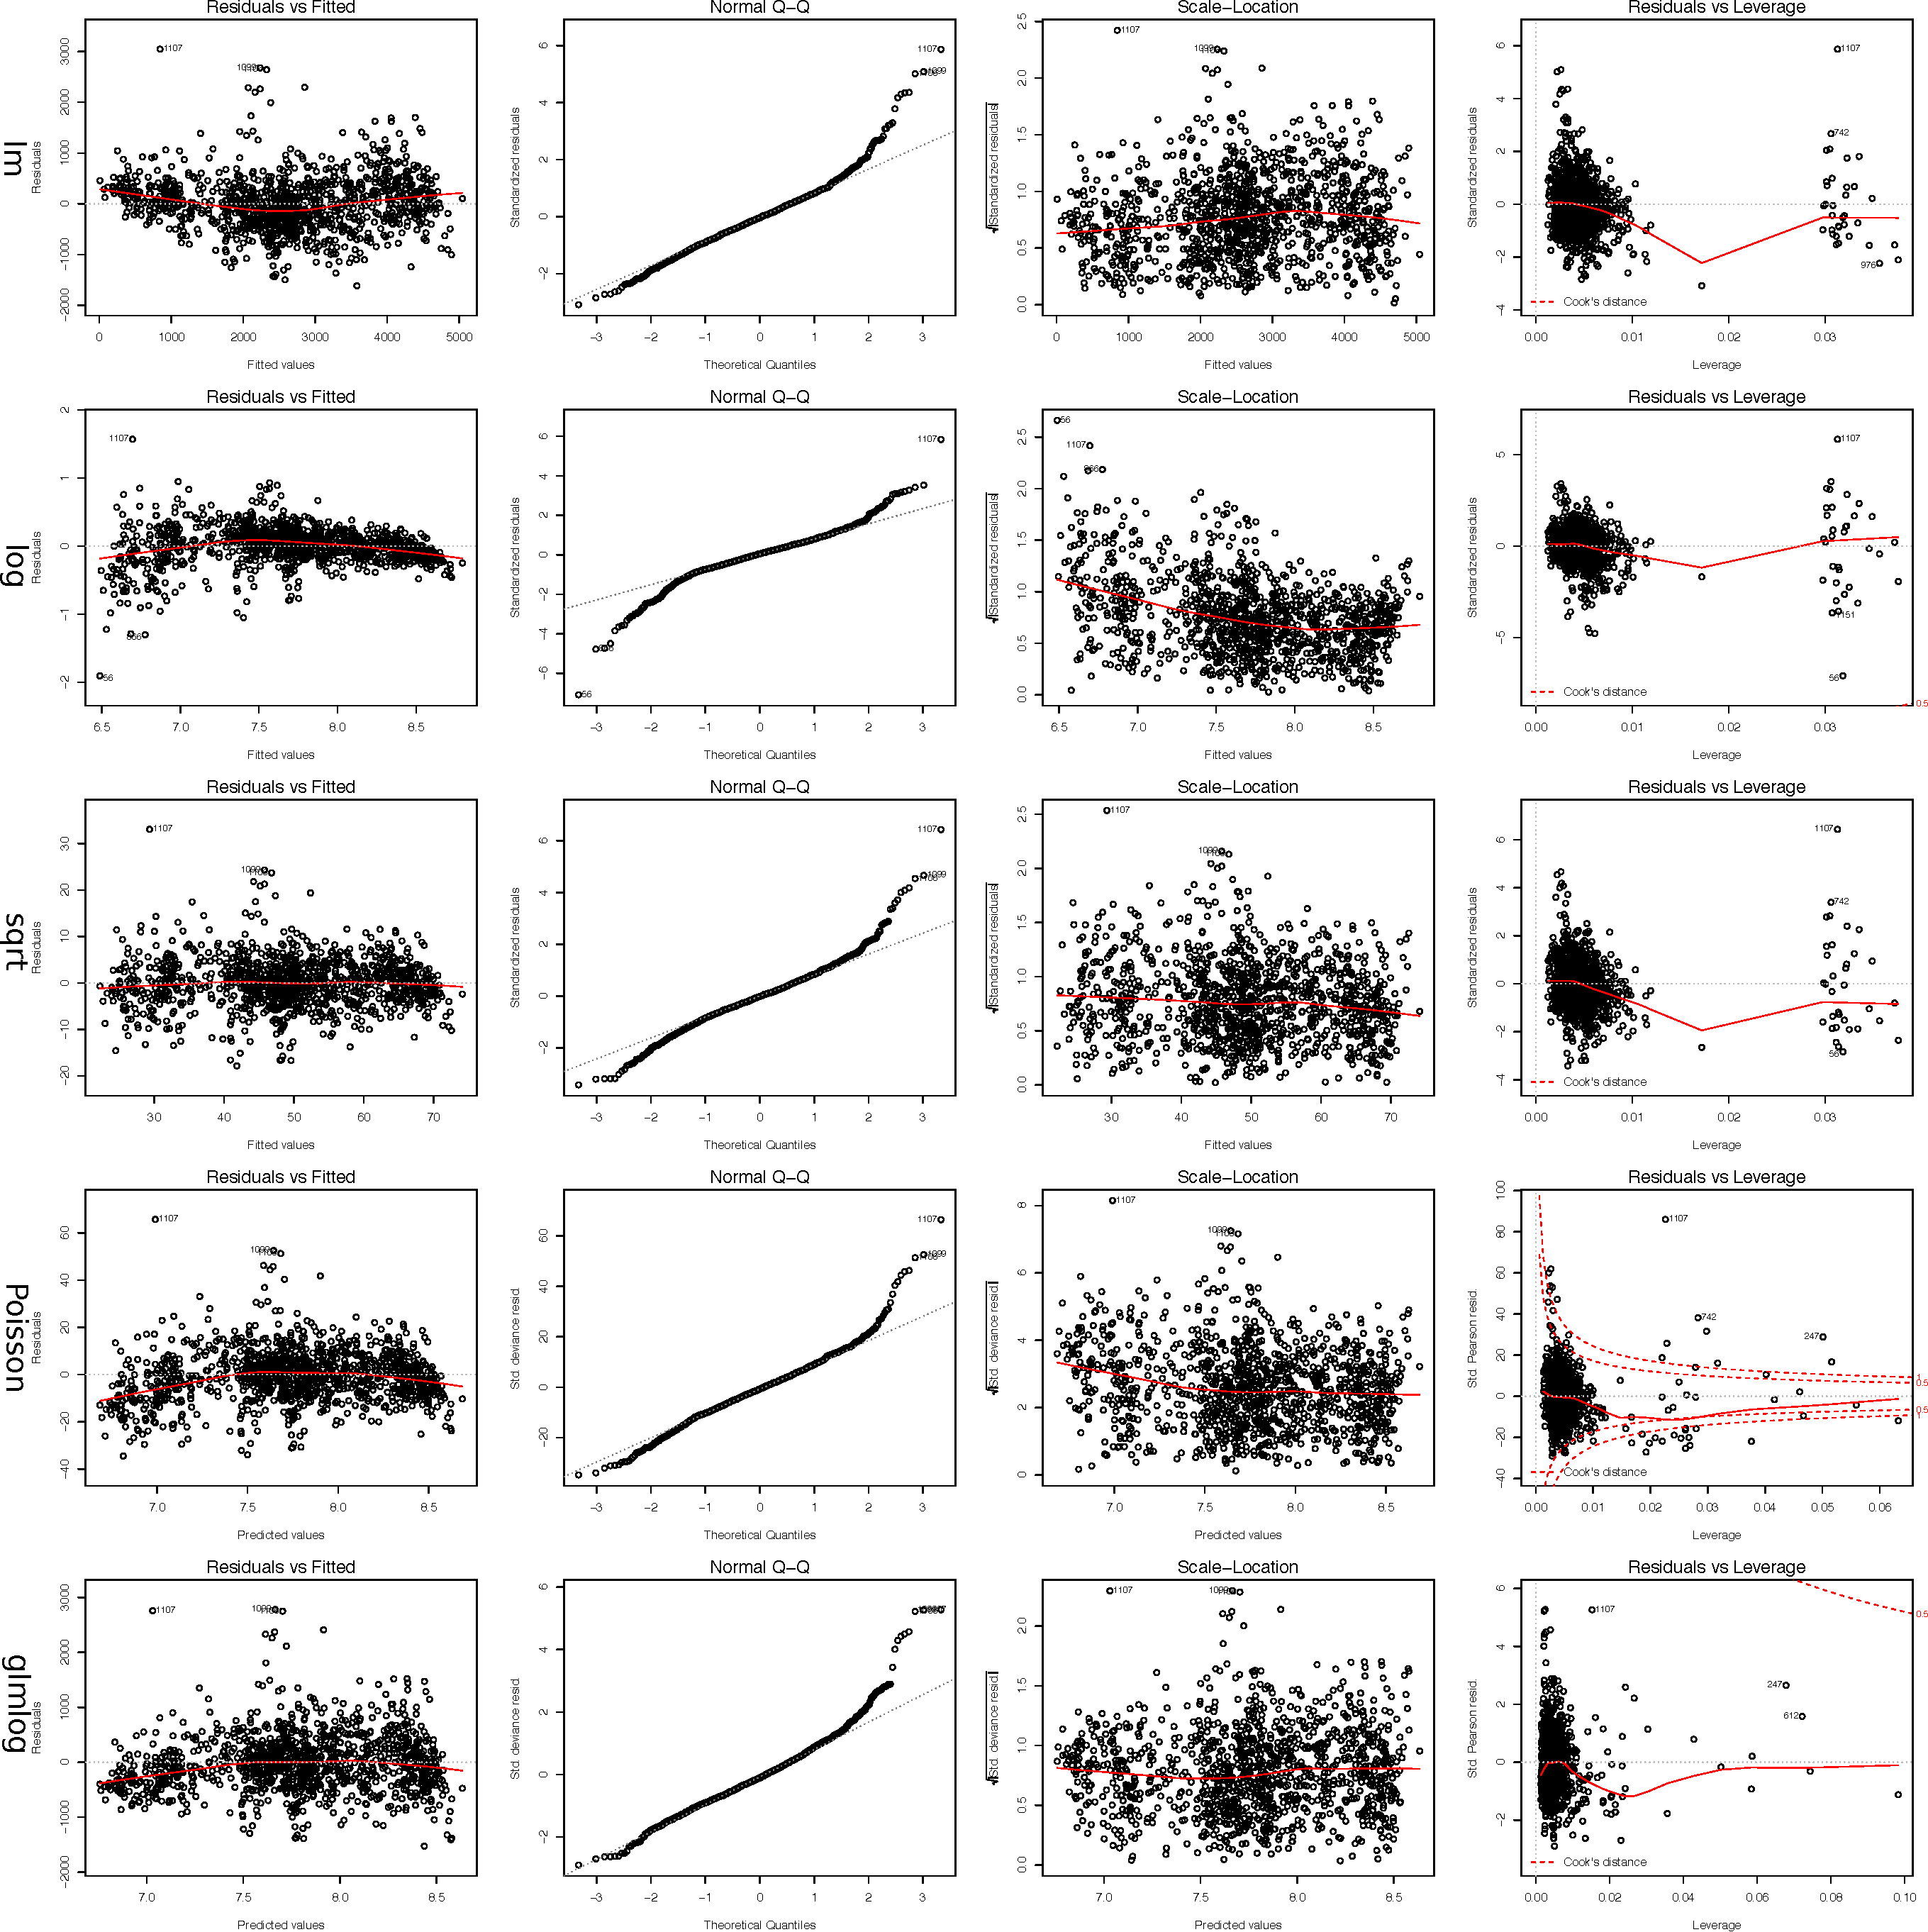
\includegraphics[width=1\textwidth]{figures/y_transform} 
  \caption{Scatterplot Matrix of covariates in the Group of Temperature and the Response}
  \label{fig:y_transform}
\end{figure*}

\subsection{Model residual analysis}

To evaluate the impact of different transformations on $Y$, the following visualization plots are used for comparison among models~\eqref{eqref:notransymodel}-\eqref{eqref:glmlog_model}.
\begin{enumerate}
\item \textbf{Residual vs. Fitted plot:} A plot of the residuals against the fitted values should show no pattern. If a pattern is observed, there may be 'heteroscedasticity' in the errors. That is, the variance of the residuals may not be constant. This indicates a transformation of the dependent variable may be required. It is shown in Figure~\ref{fig:y_transform} that the model with original bike count as dependent variable has a clear varying variance in its residual: the residual becomes larger when the bike counts to be predicted become larger. Among the four common transformations we tested (log, sqrt, Poisson and glmlog), the square root transformation results in the best residual plot, which remains constant for all fitted values. 
\item \textbf{Normal Q-Q plot:} The Normal Quantile-Quantile (Q-Q) plot represents an informal graphical test of the hypothesis that a data sequence is normally distributed. That is, if the points on a normal Q-Q plot are reasonably well approximated by a straight line, the Gaussian data hypothesis is plausible, while marked deviations from linearity provide evidence against this hypothesis~\cite{Pearson2011}. It is shown in Figure~\ref{fig:y_transform} that all models under consideration don't have a perfectly Normal distributed residuals, as is required by the linear regression models. For the square root transformation, the residual error has a slightly heavy tail on the right side. 
\item \textbf{Scale-Location plot:} It depicts the square root of the absolute values of the residuals against the fitted values, with a lowess curve helpfully overlaid. The scale-location plot is often used to check if the data possesses homoscedasticity, which is required for the linear regression model. Ideally if the modeling data has homoscedasticity, the lowess curve is expected to be flat, not sloped, and the square root of residuals should be approximately evenly distributed along the lowess curve. Using this criterion, it is shown in Figure~\ref{fig:y_transform} that the square root transformed model has the least heteroscedasticity because its lowess curve is relatively flat and the residual didn't show a obvious pattern.
\item \textbf{Residual vs. Leverage plot:} This plot depicts the standardized residuals against the leverage for each point in the data series. The Cook's Distance is also shown in the plot. This plot is mainly used to identify extreme points and possible outliers in the data series that could shift the regression line significantly. The further out in the $X$ or $Y$ axis, the more leverage or standardized residual the point in dataset has. More details on the Residual vs. Leverage plot could be found in~\cite{gung13}. From Figure~\ref{fig:y_transform} it can be seen that there are a few points in the dataset that has large leverage on the regression lines (indicated by points to the far right side of the plot). The Poisson model has relatively larger residuals with quite a few points with big Cook's distance. This indicate the Poisson model might not be a good fit. For each model, there is one point has big positive error (1107). This outlier point corresponds to the 'City Bike to Work Day' where there is more than six thousand bike passing the Fremont Bridge in one day. This suggests proper data cleaning is required (i.e., removing outliers) to best capture the relationship between utilitarian bike ridership and weather/temporal factors. 
\end{enumerate}
In summary, after exploration of different transformations of the dependent variable, the squared root of bike count appears to give the best properties of the resulting model: its residual has an approximate constant variance; it follows an approximate Gaussian distribution; it satisifies the homoscedasticity assumption of the error terms. Therefore, we use the square root transformed bike count in our following analysis. 

\newpage
\thispagestyle{empty}
\mbox{}

\section{Model Specification}

In this section, we investigate five different model specifications and conduct a detailed performance comparison by means of goodness-of-fit, cross validation, and their predictive power. 

The following five models are considered in this section:
\begin{enumerate}
\item[-] \textbf{Model 0}
\begin{align}
\log(\text{Count}_t) &= \beta_0 + \beta_1 \text{TempMaxSq}_t + \beta_2 \text{Holiday}_t + \beta_3 \text{PrecpProb}_t + \beta_4 \text{Weekend}_t \nonumber\\
&\qquad + \beta_5 \text{Daylight}_t + \beta_6 \text{UW}_t + \epsilon.\label{eqref:model0}
\end{align}
In this model, the log of bike count is used as $Y$, and the independent variables are: squared max temperature, holiday indicator, precipitation probability, weekend indicator, daylight hours, and ``UW in session'' indicator. Model 0 serves as the ``base model''. All the following models differ from the base model by changing or adding one independent variable. 
\item[-] \textbf{Model 1}
\begin{align}
\log(\text{Count}_t) &= \beta_0 + \beta_1 \text{TempMaxSq}_t + \beta_2 \text{Holiday}_t + \beta_3 \text{PrecpProb}_t + \beta_4 \text{Weekend}_t \nonumber\\
&\qquad + \beta_5 \text{Season}_t + \beta_6 \text{UW}_t + \epsilon.\label{eqref:model1}
\end{align}
Model 1 replaces the daylight hours in Model 0 by the Season indicator.
\item[-] \textbf{Model 2}
\begin{align}
\log(\text{Count}_t) &= \beta_0 + \beta_1 \text{TempMaxSq}_t + \beta_2 \text{Holiday}_t + \beta_3 \text{PrecpProb}_t + \beta_4 \text{Weekend}_t \nonumber\\
&\qquad+ \beta_5 \text{Daylight}_t + \beta_6 \text{Icon}_t + \beta_7 \text{UW}_t + \epsilon.\label{eqref:model2}
\end{align}
Model 2 add one more independent variable, the weather icon, to Model 0.
\item[-] \textbf{Model 3}
\begin{align}
\log(\text{Count}_t) &= \beta_0 + \beta_1 \text{TempMaxSq}_t + \beta_2 \text{Holiday}_t + \beta_3 \text{PrecpProb}_t +\beta_4 \text{Weekend}_t  \nonumber\\
&\qquad + \beta_5 \text{PrecpProb}_t \times \text{Weekend}_t + \beta_6 \text{Daylight}_t + \beta_7 \text{UW}_t + \epsilon. \label{eqref:model3}
\end{align}
Model 3 differs from Model 0 by allowing interactions between Precipitation Probability and the Weekend indicator variable.
\item[-] \textbf{Model 4}
\begin{align}
\log(\text{Count}_t) &= \beta_0 + \beta_1 \text{TempMaxSq}_t + \beta_2 \text{Holiday}_t + \beta_3 \text{PrecpProb}_t + \beta_4 \text{dow}_t \nonumber\\
&\qquad + \beta_5 \text{Daylight}_t + \beta_6 \text{UW}_t + \epsilon.\label{eqref:model4}
\end{align}
Model 4 replaces the weekend indicator in Model 0 by the dow indicator. 
\end{enumerate}

A summary of the model specification used in this analysis is provided in Table~\ref{tbl:model_spec}. Note that Model 0 serves as the base model in this analysis. 

\begin{table}
 \centering 
\caption{Model Specification} 
  \label{tbl:model_spec} 
\begin{tabular}{| c || c |} 
\hline 
  Name & Model Formula \\ 
\hline
  Model 0 & log(count) $\sim$ temperatureMaxSq  + holiday + precipProbability  + Wknd+ daylight +uw  \\ 
  Model 1 & log(count) $\sim$ temperatureMaxSq  + holiday +  precipProbability  + Wknd+ season +uw \\ 
  Model 2 & log(count) $\sim$ temperatureMaxSq  + holiday +  precipProbability  + Wknd+ daylight+ icon +uw\\ 
  Model 3 & log(count) $\sim$ temperatureMaxSq  + holiday +   precipProbability*Wknd + daylight +uw\\ 
  Model 4 &  log(count) $\sim$ temperatureMaxSq  + holiday +  precipProbability  + dow + daylight +uw\\ 
\hline 
\end{tabular} 
\end{table} 

\subsection{Fitted model and goodness-of-fit}
We summarize the model fitting results (including all the regression coefficients) as well as their goodness-of-fit criterion in Table~\ref{tbl:modelspec1} and Table~\ref{tbl:modelspec2}.

\begin{table}[!htbp] \centering 
  \caption{Model Comparison Results} 
  \label{tbl:modelspec1} 
\begin{tabular}{@{\extracolsep{-65pt}}lD{.}{.}{-3} D{.}{.}{-3} D{.}{.}{-3} } 
\\[-3ex]\hline 
\hline \\[-4ex] 
 & \multicolumn{3}{c}{\textit{Dependent variable: log(BikeCounts)}} \\ 
\cline{2-4} 
\\[-4ex] & \multicolumn{1}{c}{Model 0} & \multicolumn{1}{c}{Model 1} & \multicolumn{1}{c}{Model 2}\\ 
\hline \\[-4ex] 
 TempMaxSq & 0.0002^{***}$ $(0.00001) & 0.0002^{***}$ $(0.00001) & 0.0002^{***}$ $(0.00001) \\ 
  Holiday & -0.798^{***}$ $(0.046) & -0.822^{***}$ $(0.046) & -0.804^{***}$ $(0.045) \\ 
  PrecipProb & -0.493^{***}$ $(0.025) & -0.524^{***}$ $(0.025) & -0.322^{***}$ $(0.041) \\ 
  Weekend & -0.811^{***}$ $(0.017) & -0.815^{***}$ $(0.017) & -0.811^{***}$ $(0.017) \\ 
  daylight & 0.00002^{***}$ $(0.00000) &  & 0.00002^{***}$ $(0.00000) \\ 
  spring &  & 0.061^{***}$ $(0.022) &  \\ 
  summer &  & 0.064^{**}$ $(0.029) &  \\ 
  winter &  & -0.199^{***}$ $(0.025) &  \\ 
  cloudy &  &  & -0.115^{**}$ $(0.056) \\ 
  fog &  &  & 0.023$ $(0.038) \\ 
  partly-cloudy-day &  &  & 0.018$ $(0.023) \\ 
  partly-cloudy-night &  &  & 0.054^{*}$ $(0.032) \\ 
  rain &  &  & -0.139^{***}$ $(0.030) \\ 
  wind &  &  & -0.206$ $(0.184) \\ 
  UW & 0.202^{***}$ $(0.018) & 0.178^{***}$ $(0.020) & 0.200^{***}$ $(0.018) \\ 
  const. & 6.764^{***}$ $(0.047) & 7.381^{***}$ $(0.047) & 6.759^{***}$ $(0.049) \\ 
 \hline \\[-1.8ex] 
Observations & \multicolumn{1}{c}{1,157} & \multicolumn{1}{c}{1,157} & \multicolumn{1}{c}{1,157} \\ 
R$^{2}$ & \multicolumn{1}{c}{0.819} & \multicolumn{1}{c}{0.815} & \multicolumn{1}{c}{0.825} \\ 
Adjusted R$^{2}$ & \multicolumn{1}{c}{0.818} & \multicolumn{1}{c}{0.814} & \multicolumn{1}{c}{0.823} \\ 
AIC & \multicolumn{1}{c}{173.7066} & \multicolumn{1}{c}{203.1459} & \multicolumn{1}{c}{149.7224} \\ 
BIC & \multicolumn{1}{c}{214.1353} & \multicolumn{1}{c}{253.6818} & \multicolumn{1}{c}{220.4726} \\ 
\hline 
\hline \\[-3ex] 
\textit{Note:}  & \multicolumn{3}{r}{$^{*}$p$<$0.1; $^{**}$p$<$0.05; $^{***}$p$<$0.01} \\ 
\end{tabular} 
\end{table} 

\begin{table}[!htbp] \centering 
  \caption{Model Specification Results Ctnd} 
  \label{tbl:modelspec2} 
\begin{tabular}{@{\extracolsep{-65pt}}lD{.}{.}{-3} D{.}{.}{-3} D{.}{.}{-3} } 
\\[-4ex]\hline 
\hline \\[-3ex] 
 & \multicolumn{3}{c}{\textit{Dependent variable: log(BikeCounts)}} \\ 
\cline{2-4} 
\\[-4ex] & \multicolumn{1}{c}{Model 0} & \multicolumn{1}{c}{Model 3} & \multicolumn{1}{c}{Model 4}\\ 
\hline \\[-1.8ex] 
 TempMaxSq & 0.0002^{***}$ $(0.00001) & 0.0002^{***}$ $(0.00001) & 0.0002^{***}$ $(0.00001) \\ 
  Holiday & -0.798^{***}$ $(0.046) & -0.796^{***}$ $(0.044) & -0.793^{***}$ $(0.045) \\ 
  PrecipProb & -0.493^{***}$ $(0.025) & -0.359^{***}$ $(0.027) & -0.491^{***}$ $(0.024) \\ 
  Weekend & -0.811^{***}$ $(0.017) & -0.678^{***}$ $(0.021) &  \\ 
  Mon &  &  & 0.135^{***}$ $(0.028) \\ 
  Sat &  &  & -0.677^{***}$ $(0.028) \\ 
  Sun &  &  & -0.737^{***}$ $(0.028) \\ 
  Thu &  &  & 0.089^{***}$ $(0.028) \\ 
  Tue &  &  & 0.150^{***}$ $(0.028) \\ 
  Wed &  &  & 0.146^{***}$ $(0.028) \\ 
  daylight & 0.00002^{***}$ $(0.000) & 0.00002^{***}$ $(0.000) & 0.00002^{***}$ $(0.000) \\ 
  uw & 0.202^{***}$ $(0.018) & 0.201^{***}$ $(0.018) & 0.205^{***}$ $(0.018) \\ 
  PrecipProb:Wknd &  & -0.464^{***}$ $(0.048) &  \\ 
  const. & 6.764^{***}$ $(0.047) & 6.727^{***}$ $(0.045) & 6.654^{***}$ $(0.049) \\ 
 \hline \\[-1.8ex] 
Observations & \multicolumn{1}{c}{1,157} & \multicolumn{1}{c}{1,157} & \multicolumn{1}{c}{1,157} \\ 
R$^{2}$ & \multicolumn{1}{c}{0.819} & \multicolumn{1}{c}{0.832} & \multicolumn{1}{c}{0.826} \\ 
Adjusted R$^{2}$ & \multicolumn{1}{c}{0.818} & \multicolumn{1}{c}{0.831} & \multicolumn{1}{c}{0.824} \\ 
AIC & \multicolumn{1}{c}{173.7066} & \multicolumn{1}{c}{86.6983} & \multicolumn{1}{c}{139.2741} \\ 
BIC & \multicolumn{1}{c}{214.1353} & \multicolumn{1}{c}{132.1806} & \multicolumn{1}{c}{204.9707} \\ 
\hline 
\hline \\[-3ex] 
\textit{Note:}  & \multicolumn{3}{r}{$^{*}$p$<$0.1; $^{**}$p$<$0.05; $^{***}$p$<$0.01} \\ 
\end{tabular} 
\end{table} 

All fitted models confirm that the bicycle counts have a strong postive relationship with temperature, and a negative relationship with precipitation probability. During weekend and holiday, there is a significant drop in the bike counts. This makes sense since the Fremont bridge is primary a utilitarian bike facility. The daylight, or the seasons, are included to account for the seasonality in the bike count time series. With longer daylight, a larger daily bike count is observed.  

Among five models that are considered, Model 3 has the highest $R^2$, adjusted $R^2$, and the smalledst AIC and BIC values. It could be due to the fact in Model 3, the interaction item (PrecipProb:Wknd) is included to account for the nonlinear relationship between bike counts and those two factors: rather than assuming the bike count depends on the precipitation probability and weekend indicator in an independent fashion, Model 3 assumes the combination of the two jointly impact on bike ridership. This makes sense sincde for utilitarian bicyclist, it is very likely if it rains AND it is weekend, they won't go out biking, whereas in the weekdays, they will still travel even if it's rainy. For simplicity, the weekend indicator is included to substitute the day of week variable. A $R^2$ value of 0.832 indicates that 83.2\% of the variance in the bike count datasets is explained by the model fitted values. 

\textbf{To do: include model interpretation? Make model recommendation?}

%\newpage
%\thispagestyle{empty}
%\mbox{}

\section{Generalized Additive Model (GAM)}

To better explore the nonlinear relationship between the bike counts and weather factors such as temperature and precipitation, a generalized additive model (GAM) is fitted to help understand the relationship. The general GAM methodology is described in Section~\ref{sec:gamintro}. Recall that a GAM has the following form:
\begin{equation}
\log(E[\text{Count}_t]) = \beta_0 + \beta_1 f_1(\text{TempMaxSq}_t) + \beta_2 \text{Holiday}_t + \beta_3 f_2(\text{PrecipProb}_t) + \beta_4 \text{Weekend}_t + \beta_5 \text{Daylight}_t. \label{eqref:gamodel}
\end{equation}
where $f_1$ and $f_2$ are two nonlinear smooth functions of \texttt{TempMaxSq} and \texttt{PrecipProb}, respectively. A log link function is used to connect the expected bike counts with the independent variables. In this study, the \texttt{gam} function in the \texttt{mgcv} package of R is used to fit the GAM model. By default, $f_1$ and $f_2$ will take the form of the built-in nonparametric smooth splines. The smoothing parameter is chosen automatically using cross-validation.

\begin{figure}
\centering
\vspace{-1cm}
   \includegraphics[width=1\textwidth]{figures/gam_resid} 
  \caption{Residual plot and qq-plot for GAM fit.}
  \label{fig:smooth_resid}
\vspace{-1cm}
\end{figure}

The fitted GAM model is summarized in Table~\ref{gamtable}. \textbf{Add one paragraph on the GAM model summary}. As seen in Figure~\ref{fig:smooth_resid}, there is no discernable pattern in the Residual vs. Fitted value plot. Furthermore, the Normal Q-Q plot suggest that the residual follows an approximately Gaussian distribution. 

\begin{figure}
\centering
   \includegraphics[width=1\textwidth]{figures/gam.pdf} 
\vspace{-10pt}
  \caption{Smooth functions of temperatureMax and precipProbability}
  \label{fig:smooth}
\vspace{-1.05cm}
\end{figure}

We are interested to see the form of the smooth function $f_1$ and $f_2$ of temperature and precipitation probability. Figure~\ref{fig:smooth} depicts the relationship between temperature/precipitation probability and bike counts while holding all other variables in the model constant. This allows to evaluate the nature of the influence of the respective predicator, in this case temperature and precipitation, on the dependent variable bike counts. 

As seen in Figure~\ref{fig:smooth}, the smooth function of \texttt{temperatureMax} clearly follows an approximate nonlinear relationship. When the maximum daily temperature is below $40^{\circ}$F, the bike count will approximately remain the same; when it is in the range of $40^{\circ}$F and $75^{\circ}$, the bike counts monotically increases as the temperature rises. However, when the max temperature is above $75^{\circ}$F, the bike counts will start drop. It is consistent with finding that is reported in other studies~\cite{}. The use of GAM helps one to determine the important turning points. Such information can be used to set the threshold for a temperature scale variable for modeling. 

Similarly, when the precipitation probability is smaller than 0.3, there is a relatively small negative impact with respect to the bike counts. The bike count follows a nearly linear relationship with a negative slope when the precipitation probability is between 0.3 and 0.7. When the precipitation probability is higher than 0.7, the bike count will experience the fastest drop. This finding is interesting in the sense that the utilitarian biker in Seattle will generally ignore the precipitation factor when make biking decisions unless it will rain with a very high probability. It also suggests three levels of precipitation scales could be used as an alternative to the continuous precipitation probability in the bike count model.

\section{ARIMA Analysis}

In this section, the Autoregressive Integrated Moving Average (ARIMA) model is used to account for possible autocorrelation relationship in the bike count time series. A review on the general ARIMA methodolgoy is provided in Section~\ref{arimaintro}.

Following the Box-Cox approach, we first conducted the square root transformation to the dependent variable and fit a linear regression model with the same model specification as in Model 0. The standard Augemented Dickey-Fuller test and KPSS test are applied to the residuals of the fitted model. Their results are summarized in the following Table~\ref{tbl_stationarytest}. Also shown in the top plot in Figure~\ref{fig:residual_acfpcf}, there is no discernable trend or seasonality in the residual of responses. Combining all these results together, we conclude that the residual of the fitted model is stationary and no differencing is required. 

\textbf{Add the stationary test table!!!!}

The ACF, PACF plots are then investigated to examine any possible autocorrelation in the model residuals, as is shown in Figure~\ref{fig:residual_acfpcf}. The ACF and PACF plots suggest there is still significant autocorrelation that needs to be accounted for. Since there are two peaks before the PACF falls below the significance threshold, a second order autoregressive term will be included in the final model.

\begin{figure*}
   \includegraphics[width=1\textwidth]{figures/residual_acfpcf} 
  \caption{From top to bottom: the residual plots, ACF and PACF of the sqrt model residual.}
  \label{fig:residual_acfpcf}
\end{figure*}

Next, we use \texttt{auto.arima} function in the \texttt{forecast} package in \texttt{R} to automatically determine the best ARIMA model order. The chosen ARIMA model is of the order $(2,0,1)$, which is consistent of our intuition from the PACF plot. 

Finally, we implement the ARIMA$(2,0,1)$ model using \texttt{arima} in the \texttt{forecast} package in \texttt{R}. For comparison, the ARIMA$(1,1,1)$ is also implemented and their results are summarized in Table~\ref{tbl:arimacomp} with model coefficients as well as goodness-of-fit indexes. Note that we include ARIMA$(1,1,1)$ because it is the output of \texttt{auto.arima} if we explicitly allow it to explore the model spaces where differencing is permitted.

As is shown in Table~\ref{tbl:arimacomp}, ARIMA$(2,0,1)$ has a better performance compared to ARIMA$(1,1,1)$ as it has: 1) higher log likelihood, and 2) smaller AIC values. Also, the absence of differencing step is preferred because of the simplicity.

\begin{table}[!htbp] \centering 
  \caption{ARIMA Results} 
  \label{tbl:arimacomp} 
\begin{tabular}{@{\extracolsep{5pt}}lD{.}{.}{-3} D{.}{.}{-3} } 
\\[-4ex]\hline 
\hline \\[-4ex] 
 & \multicolumn{2}{c}{\textit{Dependent variable: log(BikeCounts)}} \\ 
\cline{2-3} 
\\[-3ex] & \multicolumn{1}{c}{ARIMA(2,0,1)} & \multicolumn{1}{c}{ARIMA(1,1,1)}\\ 
\hline \\[-1.8ex] 
 ar1 & 1.269^{***}$ $(0.038) & 0.355^{***}$ $(0.033) \\ 
  ar2 & -0.303^{***}$ $(0.039) &  \\ 
  ma1 & -0.879^{***}$ $(0.021) & -0.944^{***}$ $(0.017) \\ 
  intercept & 8.252^{***}$ $(0.136) &  \\ 
  temperatureMaxSq & 0.0001^{***}$ $(0.00004) & 0.0001^{***}$ $(0.00003) \\ 
  holiday & -0.681^{***}$ $(0.040) & -0.675^{***}$ $(0.019) \\ 
  precipProbability & -0.481^{***}$ $(0.024) & -0.479^{***}$ $(0.023) \\ 
  Wknd & -0.790^{***}$ $(0.016) & -0.787^{***}$ $(0.013) \\ 
  uw & 0.111^{***}$ $(0.040) & 0.137^{***}$ $(0.019) \\ 
  daylight & 0.00002 & 0.00002 \\ 
 \hline \\[-1.8ex] 
Observations & \multicolumn{1}{c}{1,157} & \multicolumn{1}{c}{1,156} \\ 
Log Likelihood & \multicolumn{1}{c}{45.906} & \multicolumn{1}{c}{37.183} \\ 
$\sigma^{2}$ & \multicolumn{1}{c}{0.054} & \multicolumn{1}{c}{0.055} \\ 
Akaike Inf. Crit. & \multicolumn{1}{c}{-69.812} & \multicolumn{1}{c}{-56.366} \\ 
\hline 
\hline \\[-1.8ex] 
\textit{Note:}  & \multicolumn{2}{r}{$^{*}$p$<$0.1; $^{**}$p$<$0.05; $^{***}$p$<$0.01} \\ 
\end{tabular} 
\end{table} 

\section{Prediction}

In this section, we are interested to evaluate the predicative power of the following models: lm model, log model, sqrt model, poisson model, glmlog model, arima log model and arima lm model. To aid the comparison, the following analysis is performed: 1) prediction intervals, 2) confidence intervals, 3) prediction vs actual plots,

First of all, we use the entire 3 years' data to train the model and plot the actual data against fitted values, as in Figure~\ref{fig:avp_fitted}.

Second, we use the first 2 years' data to train the model and then use the trained model to predict the 3rd year's bike counts. The actual vs predicted values plots are shown in Figure~\ref{fig:avp_crossvalidate}

\begin{figure*}
\includegraphics[width=1\textwidth]{figures/actualvspred.pdf}
\caption{Actual vs predicted plots}
\label{fig:avp_fitted}
\end{figure*}

\begin{figure*}
%\vspace{-40pt}
\includegraphics[width=1\textwidth]{figures/actualvsfited.pdf}
\caption{Actual vs fitted plots}
\label{fig:avp_crossvalidate}
\end{figure*}

For comparison of the predicative power, we also include the arima model for the lm model as well. See Figure~\ref{fig:avp_arima1} for cross validation and Figure~\ref{fig:avp_arima2} for fitted values.


\begin{figure*}
   \includegraphics[width=1\textwidth]{figures/actualvspred_arima} 
  \caption{Actual vs Predicted plots}
  \label{fig:avp_arima1}
\end{figure*}

\begin{figure*}
   \includegraphics[width=1\textwidth]{figures/actualvsfit_arima.pdf} 
  \caption{Actual vs Fitted plots}
  \label{fig:avp_arima2}
\end{figure*}

\newpage
\thispagestyle{empty}
\mbox{}


\section{Trend Analysis}

\begin{figure*}
\includegraphics[width=1\textwidth]{figures/trend}
\caption{Bike count trend after removing weather and seasonal factors. Note the green line is zero, red line is the linear model fit to the residual error of log model.}
\label{fig:trend}
\end{figure*}

We are also interested to reveal trend from the data. More specifically, we want to ask this question: after removing all weather and seasonality factors, does the bike count have an upward trend in the past three years? To answer this question, we fit a linear model to the residual of the log model. As is shown in Figure~\ref{fig:trend}, there is a slight upward trend of the bike count in the past three years. Since we are looking at the residual error, the weather and other seasonal factors have already been removed. The red line (linear fit to the residual) has a positive slope indicates the bike count is increasing. However, such increase is very small considering the noise in daily bike count.


%% ========== Chapter 5
% 
%\chapter{Conclusion}
 
%
% ==========   Bibliography
%
\bibliographystyle{plain}
\bibliography{bikecounts.bib}

%
% ==========   Appendices
%
\appendix
\raggedbottom\sloppy
 
% ========== Appendix A
 
\chapter{Where to find the files}
 

\vita{Jim Fox is a Software Engineer with UW Information Technology at the University of Washington.
His duties do not include maintaining this package.  That is rather
an avocation which he enjoys as time and circumstance allow.

He welcomes your comments to {\tt fox@uw.edu}.
}


\end{document}
